% questions.tex —— 2010 年·普通高等学校招生考试·湖南卷·文科 · 题目内容片段（无答案）
% 由 tools/generate_projects.py 依来源总账自 2010/2010_数学真题_湖南文_试题.md 生成，勿手改（改源 MD 后重跑）
状态：needs-review；依固定候选 PDF 两页（印刷页 603–604）逐题核验，六幅图已矢量重绘。原页未印分值，不补。
\gkpart{一、选择题}
\begin{question}
\gkti{1}复数 $\dfrac{2}{1-i}$ 等于（　）

（A）$1+i$

（B）$1-i$

（C）$-1+i$

（D）$-1-i$

\end{question}
\begin{question}
\gkti{2}下列命题中的假命题是（　）

（A）$\exists x\in\mathbf R$，$\lg x=0$

（B）$\exists x\in\mathbf R$，$\tan x=1$

（C）$\forall x\in\mathbf R$，$x^3>0$

（D）$\forall x\in\mathbf R$，$2^x>0$

\end{question}
\begin{question}
\gkti{3}某商品销售量 $y$（件）与销售价格 $x$（元/件）负相关，则其回归方程可能是（　）

（A）$\hat y=-10x+200$

（B）$\hat y=10x+200$

（C）$\hat y=-10x-200$

（D）$\hat y=10x-200$

\end{question}
\begin{question}
\gkti{4}极坐标 $\rho=\cos\theta$ 和参数方程 $\begin{cases}x=-1-t,\\ y=2+t\end{cases}$（$t$ 为参数）所表示的图形分别是（　）

（A）直线、直线

（B）直线、圆

（C）圆、圆

（D）圆、直线

\end{question}
\begin{question}
\gkti{5}设抛物线 $y^2=8x$ 上一点 $P$ 到 $y$ 轴的距离是 $4$，则点 $P$ 到该抛物线焦点的距离是（　）

（A）$4$

（B）$6$

（C）$8$

（D）$12$

\end{question}
\begin{question}
\gkti{6}若非零向量 $\boldsymbol a$，$\boldsymbol b$ 满足 $|\boldsymbol a|=|\boldsymbol b|$，$(2\boldsymbol a+\boldsymbol b)\cdot\boldsymbol b=0$，则 $\boldsymbol a$ 与 $\boldsymbol b$ 的夹角为（　）

（A）$30^\circ$

（B）$60^\circ$

（C）$120^\circ$

（D）$150^\circ$

\end{question}
\begin{question}
\gkti{7}在 $\triangle ABC$ 中，角 $A$，$B$，$C$ 所对的边长分别为 $a$，$b$，$c$，若 $\angle C=120^\circ$，$c=\sqrt2a$，则（　）

（A）$a>b$

（B）$a<b$

（C）$a=b$

（D）$a$ 与 $b$ 的大小关系不能确定

\Needspace{0.4\textheight}
\end{question}
\begingroup
\renewenvironment{question}{\Needspace{0.5\textheight}}{}
\begin{question}
\gkti{8}函数 $y=ax^2+bx$ 与 $y=\log_{\left|\frac ba\right|}x$（$ab\neq0$，$|a|\neq|b|$）在同一直角坐标系中的图象可能是（　）
\nopagebreak[4]
\begin{center}% 2010 年湖南卷文科第 8 题选项图：四个图象（A）—（D）。
% 来源 PDF：普通高考/2010/2010湖南文.pdf，SHA-256 38611c33c9da2139ad6cd4117513ee144b09a6860180eb976c446b4858ada122。
% 原页：第 1 页（A3 三栏）第 1 栏下部，书页码 603。
% 重绘依据：照原页四个小图——两曲线为 y=ax^2+bx（过原点）与 y=log_{|b/a|}x（只画 x>0）；
%   (A) 抛物线开口向上、另一根在 0 与 1 之间，对数曲线单增；
%   (B) 抛物线开口向下、另一根在 0 与 1 之间，对数曲线单增；
%   (C) 抛物线开口向下、另一根小于 -1，对数曲线单减；
%   (D) 抛物线开口向上、另一根在 -1 与 0 之间，对数曲线单减。
%   各曲线为示意曲线，仅保持原页的开口方向、根与刻度的相对位置及对数曲线单调性。
\begin{tikzpicture}[scale=0.78, semithick]

  % ============ (A) ============
  \begin{scope}
    \begin{scope}
      \clip (-1.6,-1.2) rectangle (2.55,2.4);
      \draw plot[domain=-1.15:1.45, samples=90] (\x,{2.0*\x*(\x-0.95)});
      \draw plot[domain=0.55:2.6, samples=90] (\x,{ln(\x)/ln(2)});
    \end{scope}
    \draw[->] (-1.65,0) -- (2.65,0) node[right] {$x$};
    \draw[->] (0,-1.2) -- (0,2.45) node[above] {$y$};
    \draw (-1,0.09) -- (-1,-0.09);\node[below] at (-1,-0.18) {$-1$};
    \draw (1,0.09) -- (1,-0.09);\node[below] at (1,-0.18) {$1$};
    \node[below left] at (0,-0.10) {$O$};
    \node at (0.5,-1.75) {（A）};
  \end{scope}

  % ============ (B) ============
  \begin{scope}[shift={(10.2,0)}]
    \begin{scope}
      \clip (-1.6,-1.2) rectangle (2.55,2.4);
      \draw plot[domain=-1.1:1.35, samples=90] (\x,{-2.0*\x*(\x-0.9)});
      \draw plot[domain=0.55:2.6, samples=90] (\x,{ln(\x)/ln(2)});
    \end{scope}
    \draw[->] (-1.65,0) -- (2.65,0) node[right] {$x$};
    \draw[->] (0,-1.2) -- (0,2.45) node[above] {$y$};
    \draw (-1,0.09) -- (-1,-0.09);\node[below] at (-1,-0.18) {$-1$};
    \draw (1,0.09) -- (1,-0.09);\node[below] at (1,-0.18) {$1$};
    \node[above left] at (0,0.02) {$O$};
    \node at (0.5,-1.75) {（B）};
  \end{scope}

  % ============ (C) ============
  \begin{scope}[shift={(0,-6.9)}]
    \begin{scope}
      \clip (-1.6,-1.2) rectangle (2.55,2.4);
      \draw plot[domain=-1.8:0.55, samples=90] (\x,{-2.0*\x*(\x+1.3)});
      \draw plot[domain=0.4:2.6, samples=90] (\x,{-ln(\x)/ln(2)});
    \end{scope}
    \draw[->] (-1.65,0) -- (2.65,0) node[right] {$x$};
    \draw[->] (0,-1.2) -- (0,2.45) node[above] {$y$};
    \draw (-1,0.09) -- (-1,-0.09);\node[below] at (-1,-0.18) {$-1$};
    \draw (1,0.09) -- (1,-0.09);\node[below] at (1,-0.18) {$1$};
    \node[below left] at (0,-0.10) {$O$};
    \node at (0.5,-1.75) {（C）};
  \end{scope}

  % ============ (D) ============
  \begin{scope}[shift={(10.2,-6.9)}]
    \begin{scope}
      \clip (-1.6,-1.2) rectangle (2.55,2.4);
      \draw plot[domain=-1.5:1.25, samples=90] (\x,{2.0*\x*(\x+0.9)});
      \draw plot[domain=0.4:2.6, samples=90] (\x,{-ln(\x)/ln(2)});
    \end{scope}
    \draw[->] (-1.65,0) -- (2.65,0) node[right] {$x$};
    \draw[->] (0,-1.2) -- (0,2.45) node[above] {$y$};
    \draw (-1,0.09) -- (-1,-0.09);\node[below] at (-1,-0.18) {$-1$};
    \draw (1,0.09) -- (1,-0.09);\node[below] at (1,-0.18) {$1$};
    \node[below right] at (0,-0.06) {$O$};
    \node at (0.5,-1.75) {（D）};
  \end{scope}

\end{tikzpicture}
\end{center}
\nopagebreak[4]
\end{question}
\endgroup
\gkpart{二、填空题}
\begin{question}
\gkti{9}已知集合 $A=\{1,2,3\}$，$B=\{2,m,4\}$，$A\cap B=\{2,3\}$，则 $m=$ $\underline{\qquad}$。

\end{question}
\begin{question}
\gkti{10}已知一种材料的最佳加入量在 $100$ g 到 $200$ g 之间。若用 $0.618$ 法安排实验，则第一次试点的加入量可以是 $\underline{\qquad}$ g。

\end{question}
\begin{question}
\gkti{11}在区间 $[-1,2]$ 上随机取一个数 $x$，则 $x\in[0,1]$ 的概率为 $\underline{\qquad}$。

\Needspace{0.4\textheight}
\end{question}
\begingroup
\renewenvironment{question}{\Needspace{0.5\textheight}}{}
\begin{question}
\gkti{12}下图是求实数 $x$ 的绝对值的算法程序框图，则判断框①中可填 $\underline{\qquad}$。
\nopagebreak[4]
\begin{center}% 2010 年湖南卷文科第 12 题：求实数 x 的绝对值的算法程序框图。
% 来源 PDF：普通高考/2010/2010湖南文.pdf，SHA-256 38611c33c9da2139ad6cd4117513ee144b09a6860180eb976c446b4858ada122。
% 原页：第 1 页（A3 三栏）第 2 栏中部，书页码 603。
% 重绘依据：照原页，开始→输入 x→判断框①；判断为「是」向下经「输出 x」，
%   为「否」向右再向下经「输出 -x」；两输出框合成一线后向下到「结束」。
%   判断框内原页只印「①」，不预填条件。
\begin{tikzpicture}[scale=0.95, semithick,
  every node/.style={inner sep=2pt},
  round/.style={draw, rounded corners=6pt, minimum width=1.7cm,
    minimum height=0.62cm, align=center},
  para/.style={draw, trapezium, trapezium left angle=72, trapezium right angle=108,
    minimum width=2.6cm, minimum height=0.72cm, align=center},
  dec/.style={draw, diamond, aspect=2.6, minimum width=3.0cm,
    minimum height=1.15cm, align=center},
  arr/.style={->, >=stealth}]

  \node[round] (start) at (0,8.4) {开始};
  \node[para]  (in)    at (0,7.0) {输入 $x$};
  \node[dec]   (test)  at (0,4.9) {①};
  \node[para]  (out1)  at (0,2.9) {输出 $x$};
  \node[para]  (out2)  at (4.0,2.9) {输出 $-x$};
  \node[round] (end)   at (0,1.2) {结束};

  \draw[arr] (start) -- (in);
  \draw[arr] (in) -- (test);
  \draw[arr] (test.south) -- (out1.north);
  \node[right] at (0.16,3.95) {是};
  \draw[arr] (test.east) -| (out2.north);
  \node[above] at (2.2,4.98) {否};
  \draw (out1.south) -- (0,1.9);
  \draw (out2.south) -- (4.0,1.9) -- (0,1.9);
  \draw[arr] (0,1.9) -- (end.north);
\end{tikzpicture}
\end{center}
\nopagebreak[4]
\Needspace{0.4\textheight}
\end{question}
\endgroup
\begingroup
\renewenvironment{question}{\Needspace{0.5\textheight}}{}
\begin{question}
\gkti{13}图中的三个直角三角形是一个体积为 $20$ cm$^3$ 的几何体的三视图，则 $h=$ $\underline{\qquad}$ cm。
\nopagebreak[4]
\begin{center}% 2010 年湖南卷文科第 13 题：体积 20 cm^3 的几何体的三视图。
% 来源 PDF：普通高考/2010/2010湖南文.pdf，SHA-256 38611c33c9da2139ad6cd4117513ee144b09a6860180eb976c446b4858ada122。
% 原页：第 1 页（A3 三栏）第 2 栏下部，书页码 603。
% 重绘依据：三个直角三角形——正视图直角边 5 与 h（直角在左下），
%   侧视图直角边 6 与 h（直角在左下），俯视图直角边 5、6（直角在左上，原页未标数字）；
%   h 按原页比例画出，仅示意，不表示答案。
\begin{tikzpicture}[scale=0.62, semithick]
  % 正视图：宽 5，高 h
  \draw (0,0) -- (5,0) -- (0,4) -- cycle;
  \draw[<->] (-0.7,0) -- (-0.7,4);
  \draw (-0.85,0) -- (-0.45,0);
  \draw (-0.85,4) -- (-0.45,4);
  \node[left] at (-0.95,2) {$h$};
  \draw[<->] (0,-0.7) -- (5,-0.7);
  \draw (0,-0.85) -- (0,-0.45);
  \draw (5,-0.85) -- (5,-0.45);
  \node[below] at (2.5,-0.65) {$5$};
  \node[below] at (2.5,-1.6) {正视图};

  % 侧视图：宽 6，高 h
  \draw (7.6,0) -- (13.6,0) -- (7.6,4) -- cycle;
  \draw[<->] (7.6,-0.7) -- (13.6,-0.7);
  \draw (7.6,-0.85) -- (7.6,-0.45);
  \draw (13.6,-0.85) -- (13.6,-0.45);
  \node[below] at (10.6,-0.65) {$6$};
  \node[below] at (10.6,-1.6) {侧视图};

  % 俯视图：宽 5，高 6，直角在左上
  \draw (0,-4.4) -- (5,-4.4) -- (0,-10.4) -- cycle;
  \node[below] at (2.5,-10.7) {俯视图};
\end{tikzpicture}
\end{center}
\nopagebreak[4]
\end{question}
\endgroup
\begin{question}
\gkti{14}若不同两点 $P$，$Q$ 的坐标分别为 $(a,b)$，$(3-b,3-a)$，则线段 $PQ$ 的垂直平分线 $l$ 的斜率为 $\underline{\qquad}$，圆 $(x-2)^2+(y-3)^2=1$ 关于直线 $l$ 对称的圆的方程为 $\underline{\qquad}$。

\end{question}
\begin{question}
\gkti{15}若规定 $E=\{a_1,a_2,\cdots,a_{10}\}$ 的子集 $\{a_{i_1},a_{i_2},\cdots,a_{i_n}\}$ 为 $E$ 的第 $k$ 个子集，其中 $k=2^{i_1-1}+2^{i_2-1}+2^{i_3-1}+\cdots+2^{i_n-1}$，则

（1）$\{a_1,a_3\}$ 是 $E$ 的第 $\underline{\qquad}$ 个子集；

（2）$E$ 的第 $211$ 个子集是 $\underline{\qquad}$。

\end{question}
\gkpart{三、解答题}
\begin{question}
\gkti{16}已知函数 $f(x)=\sin2x-2\sin^2x$。

（1）求函数 $f(x)$ 的最小正周期；

（2）求函数 $f(x)$ 的最大值及 $f(x)$ 取最大值时 $x$ 的集合。

\end{question}
\begin{question}
\gkti{17}为了对某课题进行研究，用分层抽样方法从三所高校 $A$，$B$，$C$ 的相关人员中，抽取若干人组成研究小组，有关数据见下表（单位：人）：

\begin{center}
\begin{tabular}{crc}
\toprule
高校 & 相关人数 & 抽取人数 \\
\midrule
$A$ & $18$ & $x$ \\
$B$ & $36$ & $2$ \\
$C$ & $54$ & $y$ \\
\bottomrule
\end{tabular}
\end{center}

（1）求 $x$，$y$；

（2）若从高校 $B$，$C$ 抽取的人中选 $2$ 人作专题发言，求这二人都来自高校 $C$ 的概率。

\Needspace{0.4\textheight}
\end{question}
\begingroup
\renewenvironment{question}{\Needspace{0.5\textheight}}{}
\begin{question}
\gkti{18}如图所示，在长方体 $ABCD-A_1B_1C_1D_1$ 中，$AB=AD=1$，$AA_1=2$，$M$ 是棱 $CC_1$ 的中点。

（1）求异面直线 $A_1M$ 和 $C_1D_1$ 所成的角的正切值；

（2）证明：平面 $ABM\perp$ 平面 $A_1B_1M$。
\nopagebreak[4]
\begin{center}% 2010 年湖南卷文科第 18 题：长方体 ABCD-A1B1C1D1，M 为棱 CC1 的中点。
% 来源 PDF：普通高考/2010/2010湖南文.pdf，SHA-256 38611c33c9da2139ad6cd4117513ee144b09a6860180eb976c446b4858ada122。
% 原页：第 2 页（A3 三栏）第 1 栏上部，书页码 604。
% 重绘依据：照原页斜二测画法，前面 BB1C1C，后面 AA1D1D 向右上平移；
%   实线为可见棱，虚线为被遮挡的三条棱 AA1、AB、AD；
%   另以实线画出 B1M 与 BM（题中两个平面的交线所在的两条线段）。
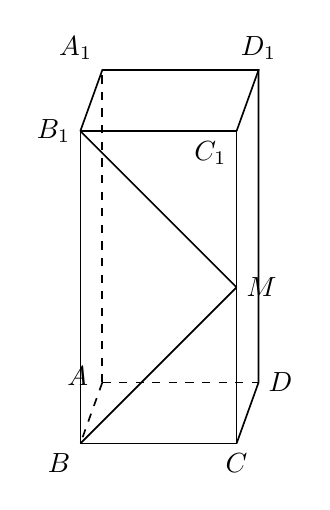
\begin{tikzpicture}[scale=0.62, semithick]
  \coordinate (B)  at (0,0);
  \coordinate (C)  at (3.2,0);
  \coordinate (C1) at (3.2,6.4);
  \coordinate (B1) at (0,6.4);
  \coordinate (A)  at (0.45,1.25);
  \coordinate (D)  at (3.65,1.25);
  \coordinate (A1) at (0.45,7.65);
  \coordinate (D1) at (3.65,7.65);
  \coordinate (M)  at (3.2,3.2);

  % 可见棱
  \draw (B) -- (C) -- (C1) -- (B1) -- cycle;
  \draw (B1) -- (A1) -- (D1) -- (C1);
  \draw (D1) -- (D) -- (C);

  % 被遮挡的棱
  \draw[dashed] (A) -- (B);
  \draw[dashed] (A) -- (D);
  \draw[dashed] (A) -- (A1);

  % 辅助线段：B1M 与 BM
  \draw (B1) -- (M);
  \draw (B) -- (M);

  \node[below left]  at (B)  {$B$};
  \node[below]       at (C)  {$C$};
  \node[left]        at (B1) {$B_1$};
  \node[below left]  at (C1) {$C_1$};
  \node[above left]  at (A1) {$A_1$};
  \node[above]       at (D1) {$D_1$};
  \node[left, xshift=-1.5pt, yshift=2.5pt]  at (A)  {$A$};
  \node[right]       at (D)  {$D$};
  \node[right]       at (M)  {$M$};
\end{tikzpicture}
\end{center}
\nopagebreak[4]
\Needspace{0.4\textheight}
\end{question}
\endgroup
\begingroup
\renewenvironment{question}{\Needspace{0.5\textheight}}{}
\begin{question}
\gkti{19}为了考察冰川的融化状况，一支科考队在某冰川上相距 $8$ km 的 $A$，$B$ 两点各建一个考察基地。视冰川面为平面形，以过 $A$，$B$ 两点的直线为 $x$ 轴，线段 $AB$ 的垂直平分线为 $y$ 轴建立平面直角坐标系（下图）。考察范围到 $A$，$B$ 两点的距离之和不超过 $10$ km 的区域。

（1）求考察区域边界曲线的方程；

（2）如图所示，设线段 $P_1P_2$ 是冰川的部分边界线（不考虑其他边界），当冰川融化时，边界线沿与其垂直的方向朝考察区域平行移动，第一年移动 $0.2$ km，以后每年移动的距离为前一年的 $2$ 倍。问：经过多长时间，点 $A$ 恰好在冰川边界线上？
\nopagebreak[4]
\begin{center}% 2010 年湖南卷文科第 19 题：冰川边界线段 P1P2 与考察区域的平面示意图。
% 来源 PDF：普通高考/2010/2010湖南文.pdf，SHA-256 38611c33c9da2139ad6cd4117513ee144b09a6860180eb976c446b4858ada122。
% 原页：第 2 页（A3 三栏）第 1 栏下部，书页码 604。
% 重绘依据：照原页坐标系，A(-4,0)、B(4,0)，冰川部分边界线为线段 P1P2，
%   P1(-5,9)、P2(-14,-3)；「已融化」「区域」标于界线左侧，「冰」「川」标于右侧。
%   原页不画考察区域（椭圆）本身，此处亦不补画。
\begin{tikzpicture}[scale=0.5, semithick, every node/.style={inner sep=2pt}]
  \draw[->] (-15.8,0) -- (7,0) node[right] {$x$};
  \draw[->] (0,-4.2) -- (0,10.6) node[above] {$y$};

  \coordinate (A)  at (-4,0);
  \coordinate (B)  at (4,0);
  \coordinate (P1) at (-5,9);
  \coordinate (P2) at (-14,-3);

  \draw (P1) -- (P2);

  \fill (A) circle (2.2pt);
  \fill (B) circle (2.2pt);
  \fill (P1) circle (2.2pt);
  \fill (P2) circle (2.2pt);

  \node[above left]  at (P1) {$P_1(-5,9)$};
  \node[below left]  at (P2) {$P_2(-14,-3)$};
  \node[below]       at (A)  {$A(-4,0)$};
  \node[below]       at (B)  {$B(4,0)$};
  \node[below left]  at (0,0) {$O$};

  % 「已融化」「区域」沿界线左侧竖排
  \node at (-6.6,7.7) {已};
  \node at (-7.6,6.2) {融};
  \node at (-8.6,4.7) {化};
  \node at (-9.8,2.9) {区};
  \node at (-10.4,1.6) {域};

  % 「冰」「川」在界线右侧
  \node at (-4.4,4.8) {冰};
  \node at (0.6,-3.0) {川};
\end{tikzpicture}
\end{center}
\nopagebreak[4]
\Needspace{0.4\textheight}
\end{question}
\endgroup
\begingroup
\renewenvironment{question}{\Needspace{0.5\textheight}}{}
\begin{question}
\gkti{20}给出下面的数表序列：
\nopagebreak[4]
\begin{center}% 2010 年湖南卷文科第 20 题：数表序列中的表 1、表 2、表 3。
% 来源 PDF：普通高考/2010/2010湖南文.pdf，SHA-256 38611c33c9da2139ad6cd4117513ee144b09a6860180eb976c446b4858ada122。
% 原页：第 2 页（A3 三栏）第 2 栏上部，书页码 604。
% 重绘依据：照原页无框格排版，表 1、表 2、表 3、⋯ 自左向右并列；
%   表 1 为 1；表 2 为「1 3」与「4」；表 3 为「1 3 5」「4 8」「12」，各行左对齐。
\begin{tikzpicture}[scale=0.95, semithick, every node/.style={inner sep=1.5pt}]

  % 表头
  \node at (0,0) {表 1};
  \node at (2.4,0) {表 2};
  \node at (5.4,0) {表 3};
  \node at (7.7,0) {$\cdots$};

  % 第 1 行
  \node at (0,-1.0) {1};
  \node at (2.0,-1.0) {1};
  \node at (3.0,-1.0) {3};
  \node at (4.7,-1.0) {1};
  \node at (5.5,-1.0) {3};
  \node at (6.3,-1.0) {5};

  % 第 2 行
  \node at (2.0,-1.8) {4};
  \node at (4.7,-1.8) {4};
  \node at (5.5,-1.8) {8};

  % 第 3 行
  \node at (4.7,-2.6) {12};

\end{tikzpicture}
\end{center}
\nopagebreak[4]
其中表 $n$（$n=1,2,3,\cdots$）有 $n$ 行，第 $1$ 行的 $n$ 个数是 $1,3,5,\cdots,2n-1$，从第 $2$ 行起，每行中的每个数都等于它肩上的两数之和。

（1）写出表 $4$，验证表 $4$ 各行中数的平均数按从上到下的顺序构成等比数列，并将结论推广到表 $n$（$n\geqslant3$）（不要求证明）；

（2）每个数列中最后一行都只有一个数，它们构成数列 $1,4,12,\cdots$，记此数列为 $\{b_n\}$，求和：$\dfrac{b_3}{b_1b_2}+\dfrac{b_4}{b_2b_3}+\cdots+\dfrac{b_{n+2}}{b_nb_{n+1}}$（$n\in\mathbf N^*$）。

\end{question}
\endgroup
\begin{question}
\gkti{21}已知函数 $f(x)=\dfrac ax+x+(a-1)\ln x+15a$，其中 $a<0$，且 $a\neq-1$。

（1）讨论函数 $f(x)$ 的单调性；

（2）设函数 $g(x)=\begin{cases}\left(-2x^3+3ax^2+6ax-4a^2-6a\right)\mathrm e^x,&x\leqslant1,\\ \mathrm e\cdot f(x),&x>1,\end{cases}$（$\mathrm e$ 是自然数的底数）。是否存在 $a$，使 $g(x)$ 在 $[a,-a]$ 上为减函数？若存在，求 $a$ 的取值范围；若不存在，请说明理由。

\end{question}